\section{The Racialized Axis: Black Family Destruction as Structural Output}

The gender-war analysis cannot stop at the dyadic interface between men and women. On the racialized axis, the same contract-collapse dynamic produces family dissolution at catastrophic scale, but with one critical difference: the state is not merely a passive referee of ambiguous obligations. It is an active participant in dissolving Black families through incarceration, environmental poisoning, predatory debt, and bureaucratic demolition. This section synthesizes peer-reviewed federal and longitudinal data to show that Black family instability is not a cultural pathology produced by deficient gender roles. It is a structural output of policy designed to extract from, and simultaneously blame, the populations it disables.

For the full formal framework mapping these empirical findings onto the five-tier extraction architecture ($E$, $P_{\text{uppet}}$, $F_{\text{enforce}}$, $I_{\text{buffer}}$, $O_{\text{racialized}}$), see Chapter~8 of \textit{The Original Power} (``The Terminal Output: Black Family Dissolution as Five-Tier Execution'').

\subsection{The False Dichotomy: Men vs.\ Women as Opposing Forces}

The public conversation about Black family instability is usually framed as a gendered blame game: Are Black men irresponsible? Are Black women too demanding, too independent, or exploiting welfare? This framing is analytically bankrupt. The peer-reviewed data show that Black men and Black women are not opposing each other in a culture war; they are sinking together under the same structural weight, with the state standing on the rope.

The correct analytical frame is \textit{structural reciprocity}: the same forces that push Black men out of households---incarceration, unemployment, environmental neurotoxicity---are the same forces that push Black women into solo parenting---partner incarceration, poverty, pregnancy complications from lead exposure. The ``tension'' between Black men and women is not a cause of family breakdown; it is a symptom of shared structural violence.

\begin{figure}[htbp]
  \centering
  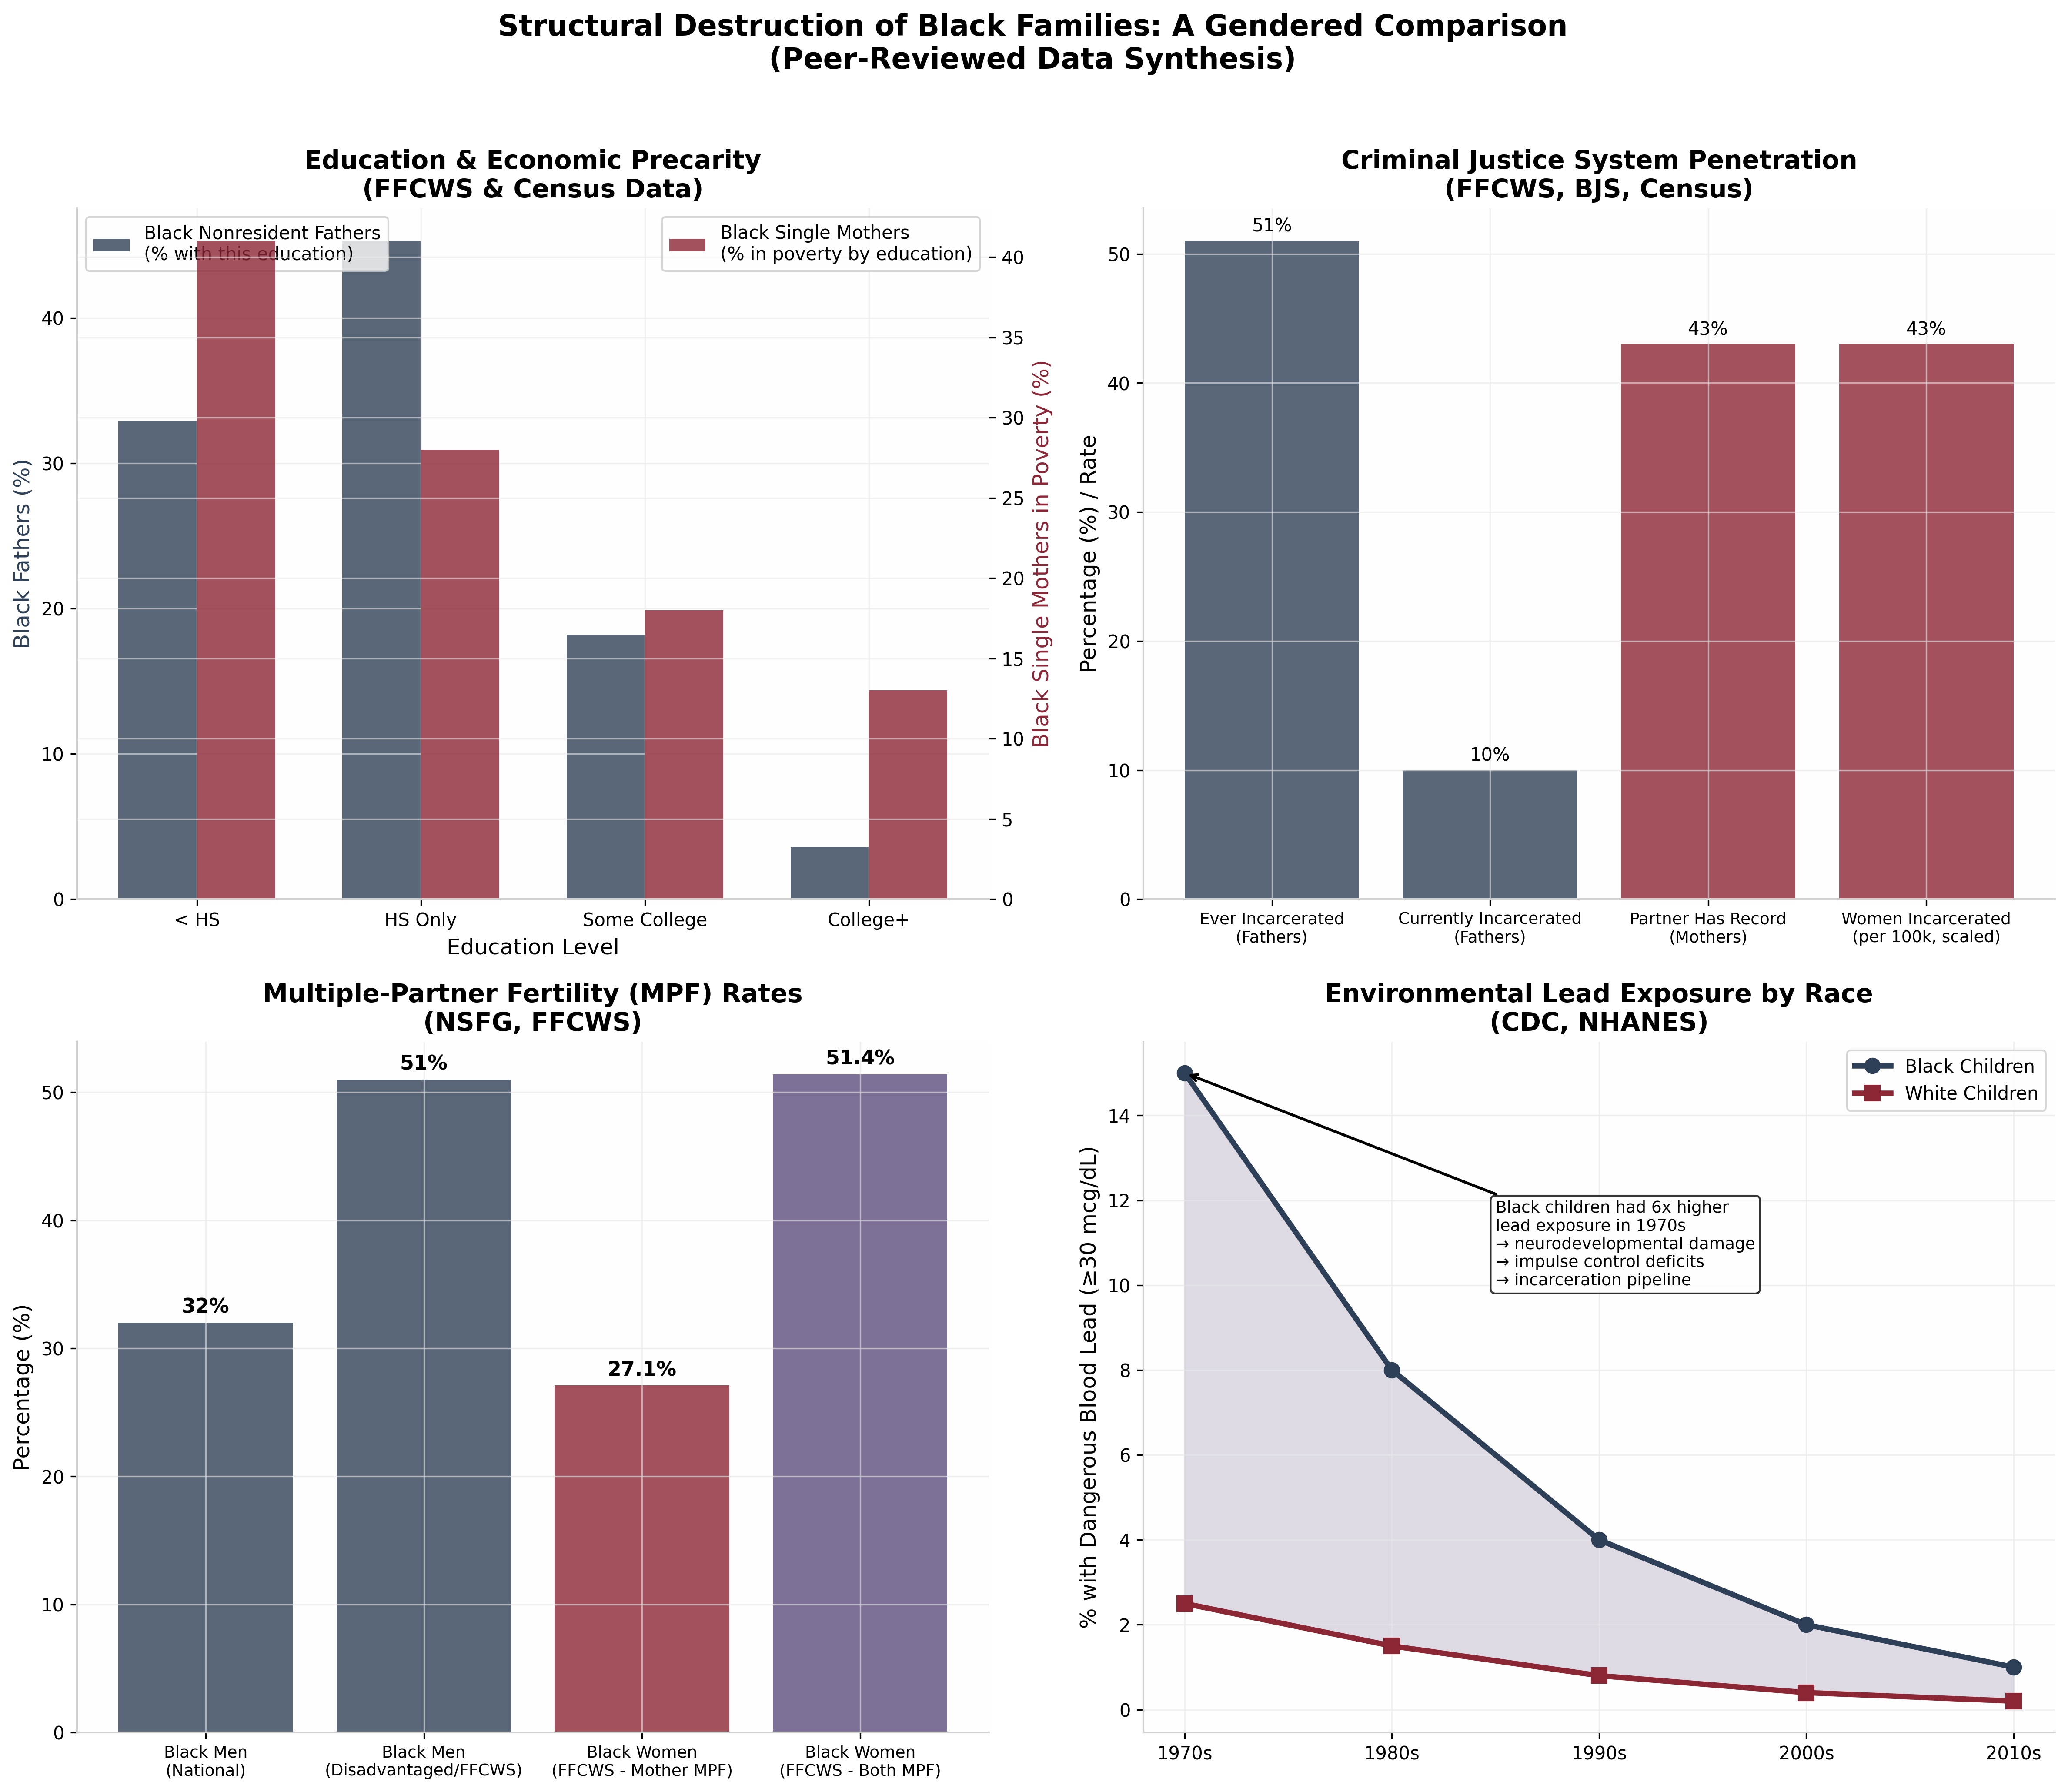
\includegraphics[width=\textwidth]{figures_black_family_structural_comparison.png}
  \caption{Structural Destruction of Black Families: A Gendered Comparison. Sources: FFCWS, BJS, Census, CDC NHANES, NSFG. The four panels show education and economic precarity (nonresident fathers and single mothers), criminal justice penetration, multiple-partner fertility rates, and environmental lead exposure disparities by race.}
  \label{fig:black_family_structural}
\end{figure}

\subsection{Comparative Anatomy of the Crisis}

\subsubsection{Education and Economics: The Mirror, Not the Ladder}

For Black men, education is a steep protective factor against multiple-partner fertility (MPF) and nonresident fatherhood. Nationally, 78\% of nonresident Black fathers in the Fragile Families and Child Wellbeing Study (FFCWS) had a high school diploma or less; only 3.6\% had a college degree. Black men with bachelor's degrees have dramatically lower rates of nonmarital first births.

For Black women, education is also protective against poverty, but the gradient is less steep for MPF itself. In the FFCWS, mother's education was not significantly associated with having children by multiple fathers after controlling for other variables. What did predict MPF for women was having worked in the year before the focal birth---suggesting they were already supporting children from prior relationships---and lower religiosity.

Both sexes face an education premium, but for women the economic return to education is blunted by the earnings penalty of single motherhood. Black single mothers with full-time jobs earn a median of \$38,000 vs.~\$50,000 for white single mothers. Even controlling for occupation and education, Black single mothers remain slightly more likely to be poor---largely because they are more likely to qualify for welfare due to structural disadvantage, not because they ``choose'' dependency.\SourceNote{Pew Research Center and Census Bureau earnings data; FFCWS demographic profiles.}

For Black women, MPF is predicted less by education than by economic activity and social context: mothers who worked in the year before the focal birth were more likely to have MPF (likely because they were already supporting children from prior relationships), and more religious mothers were less likely to have MPF.\SourceNote{FFCWS MPF correlates; Carlson and Furstenberg analyses.}

The partner pool is so structurally damaged that individual educational attainment cannot fully protect against family instability. A Black man with some college still faces a 32\% probability of a nonmarital first birth---higher than a white man who dropped out of high school (28\%).\SourceNote{NLSY79 analysis of nonmarital first births by race and education.}

\subsubsection{Criminal Justice: The Wedge Driven Between Partners}

This is where the gendered comparison reveals the state's central role. For Black men: 51\% had been incarcerated by their child's 5th birthday in the FFCWS sample. Forty-three percent of Black fathers had criminal records vs.~29\% of white fathers. The offenses were disproportionately non-violent: drugs (23.8\%), property (21.8\%), and public order/weapons (10.3\%). Only 10.9\% were for homicide or sexual assault. Current incarceration reduces father-child contact by 5.5 days per month and child support contributions by \$1,300--\$3,700/year.\SourceNote{BJS parent-prisoner data; FFCWS incarceration and child support analyses.}

For Black women, only 2.3\% of women in state prisons are there for violent offenses; most are incarcerated for drug or property crimes tied to poverty and survival. But the larger criminal justice exposure for women is vicarious: their partners. Because Black women partner with Black men, they inherit the downstream effects of mass incarceration. When a father is incarcerated, the mother becomes a de facto single mother. When he returns with debt, unemployment, and trauma, the relationship often dissolves.

The criminal justice system does not just punish individuals; it punishes couples. It removes men from households, destroys their earnings capacity, and then blames them for being absent. It leaves women holding the full weight of parenting, then blames them for being ``strong'' or ``unmarriageable.'' The system creates the conditions it then moralizes about.

\subsubsection{Multiple-Partner Fertility: The Shared Outcome}

The basic math complicates any ``small subset'' theory. According to the CDC's National Survey of Family Growth (2015--2019), 54\% of Black men aged 15--49 have no children at all; only 46\% are fathers.\SourceNote{CDC NSFG 2015--2019.} Nationally, about 17\% of all fathers and 23\% of fathers with two or more children have MPF; among younger fathers (25--32) with two or more children, the rate rises to 32\%. In the NLSY97 cohort, 48\% of men who were unmarried or nonresident at first birth had MPF by ages 23--27.\SourceNote{NSFG 2002 and 2015--2019; NLSY97 MPF analyses.}

For Black men specifically: 32\% nationally have children with more than one woman; in disadvantaged samples such as Fragile Families, 51\% do. MPF is strongly predicted by incarceration history (61\% of MPF men have served time vs.~28\% of single-partner men) and drug use.\SourceNote{NSFG 2002; FFCWS MPF analyses.}

For Black women: In the FFCWS, 27.1\% of Black mothers had children by another father; 51.4\% had MPF when both parents did. Critically, mother's MPF was not predicted by her own education but by the father's characteristics and relationship instability.

MPF is not a ``male problem'' or a ``female problem.'' It is a relationship-instability problem produced by the same structural forces. When the state removes men from households via incarceration, when it traps them in unpayable child support debt, when it exposes both partners to lead-induced aggression and impulse control deficits, the result is serial unions and overlapping fertility. MPF is the demographic footprint of structural family dissolution, not individual promiscuity.

\subsubsection{Environmental Lead: The Hidden Variable That Explains ``Violence''}

For Black men: In the 1970s, 15\% of Black children had blood lead $\geq$30 mcg/dL vs.~2.5\% of white children---a 6$\times$ disparity. Black children had 2.2$\times$ higher lead levels in utero and postnatally. Systematic reviews confirm that early lead exposure predicts adult criminal behavior, aggression, and poor impulse control.\SourceNote{CDC NHANES; NIH/PMC systematic review on lead and criminal behavior.}

For Black women: Lead stored in bone is re-mobilized during pregnancy, crossing the placenta and increasing risk of miscarriage, stillbirth, preterm birth, and low birth weight. Black pregnant persons are disproportionately exposed due to older housing and poverty.

Lead is the perfect metaphor for how the state destroys Black families: it is invisible, it is toxic, it is produced by policy (housing segregation, highway placement, disinvestment), and it is blamed on the victims. When lead-exposed boys grow into ``violent'' men, we incarcerate them. When lead-exposed women lose pregnancies or have preterm births, we blame their ``lifestyle.'' The state created the poison; the culture blames the poisoned.

\subsubsection{The Structural Mirror: A Side-by-Side Summary}

The peer-reviewed data do not support a ``small subset of irresponsible Black men'' theory. Instead, they reveal cascading structural disadvantage that hits both sexes from different angles.

\begin{center}
\small
\begin{tabular}{p{2.4cm}p{5.0cm}p{5.0cm}}
\toprule
\textbf{Factor} & \textbf{Black Men} & \textbf{Black Women} \\
\midrule
\textbf{Education} & Strong protective against MPF; 78\% of nonresident fathers have HS or less & Protective against poverty; MPF itself not strongly predicted by education \\
\addlinespace
\textbf{Crime/CJ} & 61\% of MPF men ever incarcerated; offenses mostly non-violent (drugs/property) & 58\% of incarcerated women are single mothers; partners' incarceration is the larger driver of single motherhood \\
\addlinespace
\textbf{Financials} & Mean earnings \$16K (FFCWS); 75\% in poor samples earn $<$\$500/mo or unemployed & Median \$38K full-time; 28\% poverty rate; 74.7\% have no emergency savings \\
\addlinespace
\textbf{Lead} & Childhood exposure $\rightarrow$ impulse/aggression $\rightarrow$ incarceration $\rightarrow$ family separation & Childhood + current exposure $\rightarrow$ pregnancy complications, fetal loss, preterm birth $\rightarrow$ family stress \\
\bottomrule
\end{tabular}
\end{center}

\subsection{The State's Machinery of Destruction}

The peer-reviewed data reveal at least four state mechanisms that actively dissolve Black families:

\begin{enumerate}
  \item \textbf{Mass incarceration as family dissolution.} With 51\% of African American fathers in the FFCWS experiencing incarceration by their child's 5th birthday, the criminal justice system functions as a marriage and family dissolution engine. It removes earners, traumatizes partners, and criminalizes the behaviors (drug use, property crimes, public order violations) that poverty produces.
  
  \item \textbf{Child support as a debt trap.} About 70\% of the \$113.5 billion in outstanding child support arrears nationwide is held by men earning \$10,000 or less per year. The child support system assigns unpayable orders to poor fathers. In one Mississippi sample of mostly Black fathers, 86\% were unemployed but ordered to pay \$281/month; they paid only 38\% of what was owed. Eighty-two percent had driver's licenses suspended; 45\% were held in contempt. This does not ``support children''; it criminalizes poverty, makes employment harder, and drives fathers underground.\SourceNote{National child support debt data; qualitative child support debt study, Mississippi.}
  
  \item \textbf{Housing segregation $\rightarrow$ lead $\rightarrow$ ``crime.''} Federal housing policy (redlining, highway construction, public housing placement) concentrated Black families in the oldest, most dilapidated housing stock. This produced the lead exposure gap, which produced the neurodevelopmental damage that produced the ``crime'' that justifies incarceration. It is a closed feedback loop where the state creates the problem, punishes the symptoms, and blames the culture.
  
  \item \textbf{Welfare policy and marriage penalties.} Welfare programs often include marriage penalties where benefits are reduced or eliminated if a partner moves in or if paternity is formally established. This creates a perverse incentive for informal unions and nonresident fatherhood. Meanwhile, marriage-promotion programs (funded at \$750 million federally under the Bush administration) failed to increase marriage rates because they addressed culture while ignoring structure.\SourceNote{Federal marriage-promotion program evaluations.}
\end{enumerate}

\subsection{Media Misdiagnosis: Culture vs.\ Structure}

The media narrative inverts the causal arrow. It treats Black family instability as a cultural failure that produces structural outcomes, when the peer-reviewed data show it is a structural failure that produces cultural adaptations.

\subsubsection{The Moynihan Inheritance}

The 1965 Moynihan Report framed Black family breakdown as a ``tangle of pathology'' rooted in matriarchy and absent fathers. This set the template for sixty years of coverage. The media still asks: ``Why don't Black men marry?'' and ``Why do Black women have children out of wedlock?'' It rarely asks: ``Why does the state incarcerate half of Black fathers?'' or ``Why does the EPA allow Black children to be poisoned at 6$\times$ the rate of white children?''

\subsubsection{``Deadbeat Dad'' as Moral Category}

The CDC data show that Black fathers are the most involved fathers in America when living with children, and nonresident Black fathers maintain more contact than white or Hispanic nonresident fathers.\SourceNote{CDC National Health Statistics Report, NSFG 2006--2010; 2017--2019 NSFG confirmation by Institute for Family Studies.}

Among fathers living with their children, Black fathers outperform white and Hispanic fathers on nearly every daily measure of hands-on care:
\begin{center}
\small
\begin{tabular}{lccc}
\toprule
\textbf{Daily Activity} & \textbf{Black Fathers} & \textbf{White Fathers} & \textbf{Hispanic Fathers} \\
\midrule
Bathe, dress, or diaper & 70\% & 60\% & 45\% \\
Eat meals with child & 78\% & 74\% & 64\% \\
Help with homework & 41\% & 28\% & 29\% \\
Take to/from activities & 27\% & 20\% & --- \\
\bottomrule
\end{tabular}
\end{center}

For nonresident fathers, 59\% of Black nonresident fathers see their children at least once a week, compared to only 39\% of white and 35\% of Hispanic nonresident fathers.\SourceNote{CDC NSFG 2006--2010; Institute for Family Studies analysis of 2017--2019 NSFG.} The ``deadbeat'' label is applied to men who are structurally excluded from households, not men who voluntarily abandoned them. The media never reports the 61\% incarceration rate among MPF men as the primary driver of absence; it reports the absence as a moral choice.

\subsubsection{``Welfare Queen'' as Moral Category}

Black single mothers are framed as exploiting the system or as having ``chosen'' single motherhood. The data show that 74.7\% of Black single mothers in college cannot come up with \$2,000 in an emergency, and 69.4\% do not graduate within six years. These are not women ``gaming the system''; they are women trapped by it. The welfare benefits are too low to escape poverty and too precarious to risk formalizing a partner's presence.\SourceNote{Single mother college completion and emergency savings data.}

\subsection{The AI + DOGE Double Shock}

The 2020--2026 period is not a continuation of the old story. It is an acceleration of the structural destruction already mapped, with two new blades: AI-driven labor displacement and state-administered employment demolition.

\subsubsection{The Tech Layoff Wave and Black Worker Displacement}

Black men are underrepresented in the high-paying tech roles being cut; they are overrepresented in the lower-wage, high-risk service and administrative roles that AI is replacing first. AI automation risk is highest in customer service (85\%) and office/administrative support (76\%)---sectors where Black workers are concentrated.\SourceNote{AI displacement risk studies; Sam Altman public statements on customer service elimination.}

\subsubsection{DOGE: The State Is Eating Its Own Safety Net}

Federal employment has been the single most reliable wealth-building engine for Black families because it offered what the private sector denied: anti-discrimination enforcement, union protections, defined-benefit pensions, and predictable schedules. Eighteen and a half percent of the federal workforce is Black (vs.~12\% of civilian employment). Black workers make up 36\% of the Department of Education and 36\% of HUD---double their workforce share.\SourceNote{Federal workforce demographic data.}

The DOGE cuts have been demographically targeted. Between February and July 2025, Black women lost 319,000 jobs. Black women were 33\% of federal job cuts despite being only $\sim$12\% of the federal workforce. Over the same period: White women gained 142,000 jobs; Hispanic women gained 176,000; White men gained 365,000.\SourceNote{Bureau of Labor Statistics labor force changes, Feb--July 2025.}

This is not a ``recession.'' It is a state-engineered extraction from the one employment sector that had partially offset private-sector discrimination.

\begin{figure}[htbp]
  \centering
  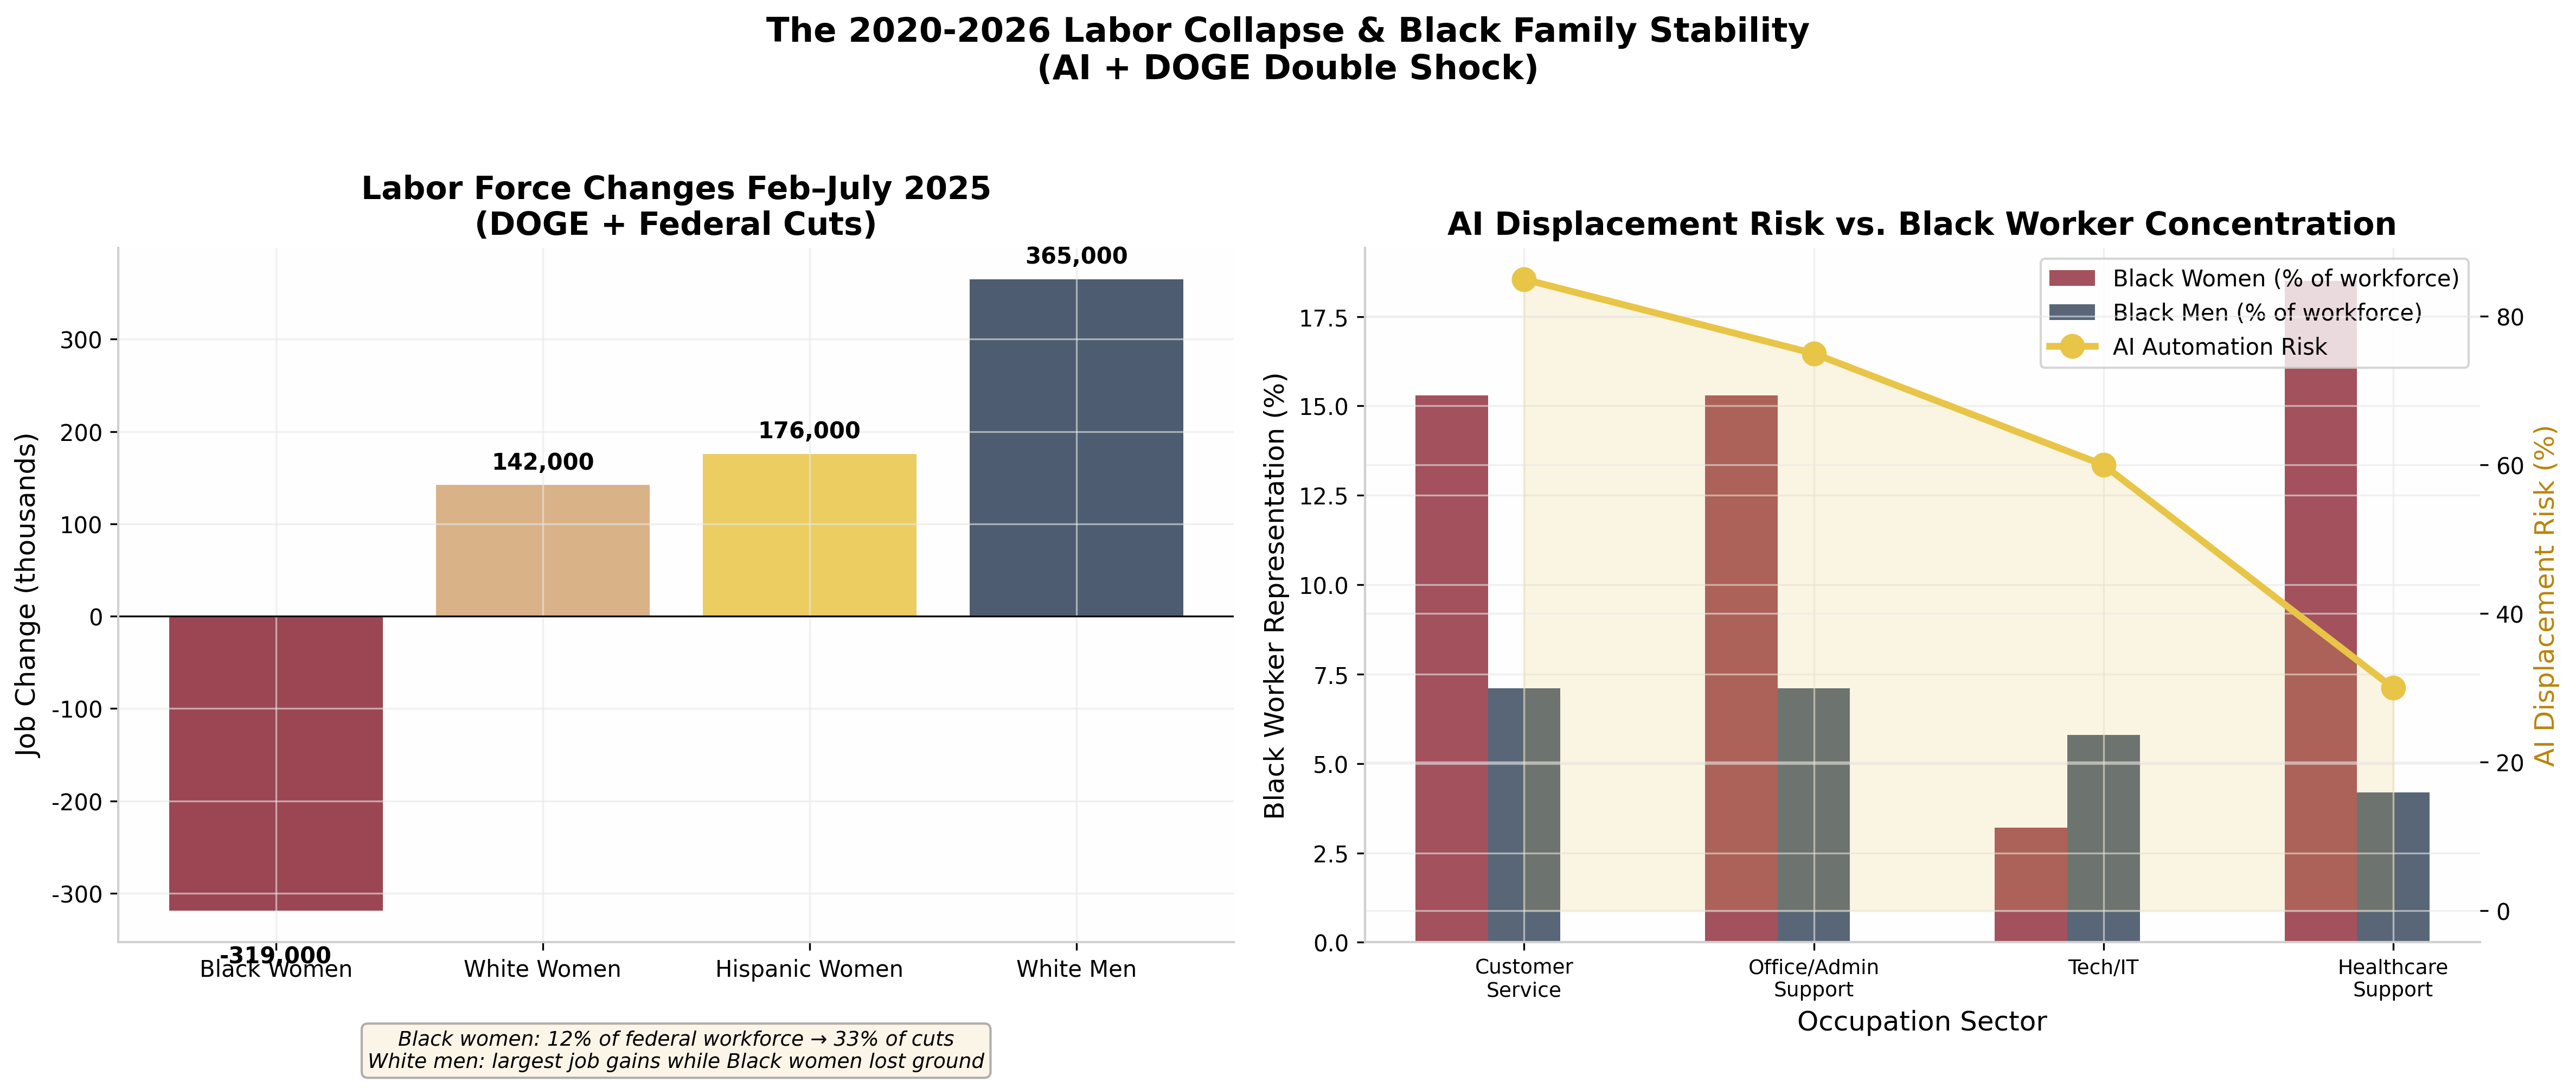
\includegraphics[width=\textwidth]{figures_ai_doge_labor_collapse.png}
  \caption{The 2020--2026 Labor Collapse and Black Family Stability (AI + DOGE Double Shock). Left panel: labor force changes February--July 2025 by demographic group. Right panel: AI displacement risk vs.\ Black worker concentration by occupation sector.}
  \label{fig:ai_doge_labor}
\end{figure}

\subsubsection{What This Means for Family Formation}

The peer-reviewed predictors of MPF and single parenthood---unemployment, earnings loss, incarceration, housing instability---are all being intensified by this double shock. When 300,000+ Black women lose federal jobs and Black men face AI displacement from service sectors, the result is not ``men not wanting to marry.'' It is couples who cannot form stable households because both partners' incomes are being systematically removed.

\subsection{MPF, ENM, and the Cooperative Kinship Hypothesis}

The nuclear family model was imposed, not chosen. Freedman's Bureau agents broke up plural and non-monogamous unions among formerly enslaved people, requiring Black men to ``select one wife'' and prosecuting the others for fornication. The nuclear family assumes one male breadwinner with stable employment, one female caregiver with stable housing, and state-provided benefits flowing through the male head of household. All three assumptions are structurally false for Black families in America.

Research by Christina Cross shows that Black children in two-parent nuclear families have outcomes comparable to white children in single-parent families---because the Black two-parent family still lacks the wealth, neighborhood quality, and institutional support that make the nuclear family functional for white Americans.\SourceNote{Christina Cross, \textit{Inherited Inequality}.} In other words: the nuclear family does not fix racial inequality because the nuclear family was designed for people who already have racial privilege.

\subsubsection{What the MPF Data Allow}

The Fragile Families data give us a natural experiment in shadow polyamory. We know that MPF is associated with family chaos (residential instability, material hardship, work instability), but when these chaos variables are controlled, the direct link between MPF and poor coparenting largely disappears. High-quality coparenting---not family structure---predicts the best child outcomes (lowest behavior problems, highest empathy). Twenty percent of coparents in Black single-mother families provide care equivalent to mothers on discipline, transportation, meals, and monitoring. Black parents have higher initial coparenting quality after dissolution than other racial groups, suggesting the fracture is relational, not cultural.\SourceNote{FFCWS coparenting and child outcome analyses.}

If the harms of MPF come from secrecy, competition, and resource scarcity rather than from the mere fact of multiple partners, then a named, cooperative, non-competitive multi-partner network should produce outcomes closer to ``high-quality coparenting'' than to ``chaotic MPF.'' The structure already exists; the variable being changed is stigma $\rightarrow$ explicitness.

\begin{figure}[htbp]
  \centering
  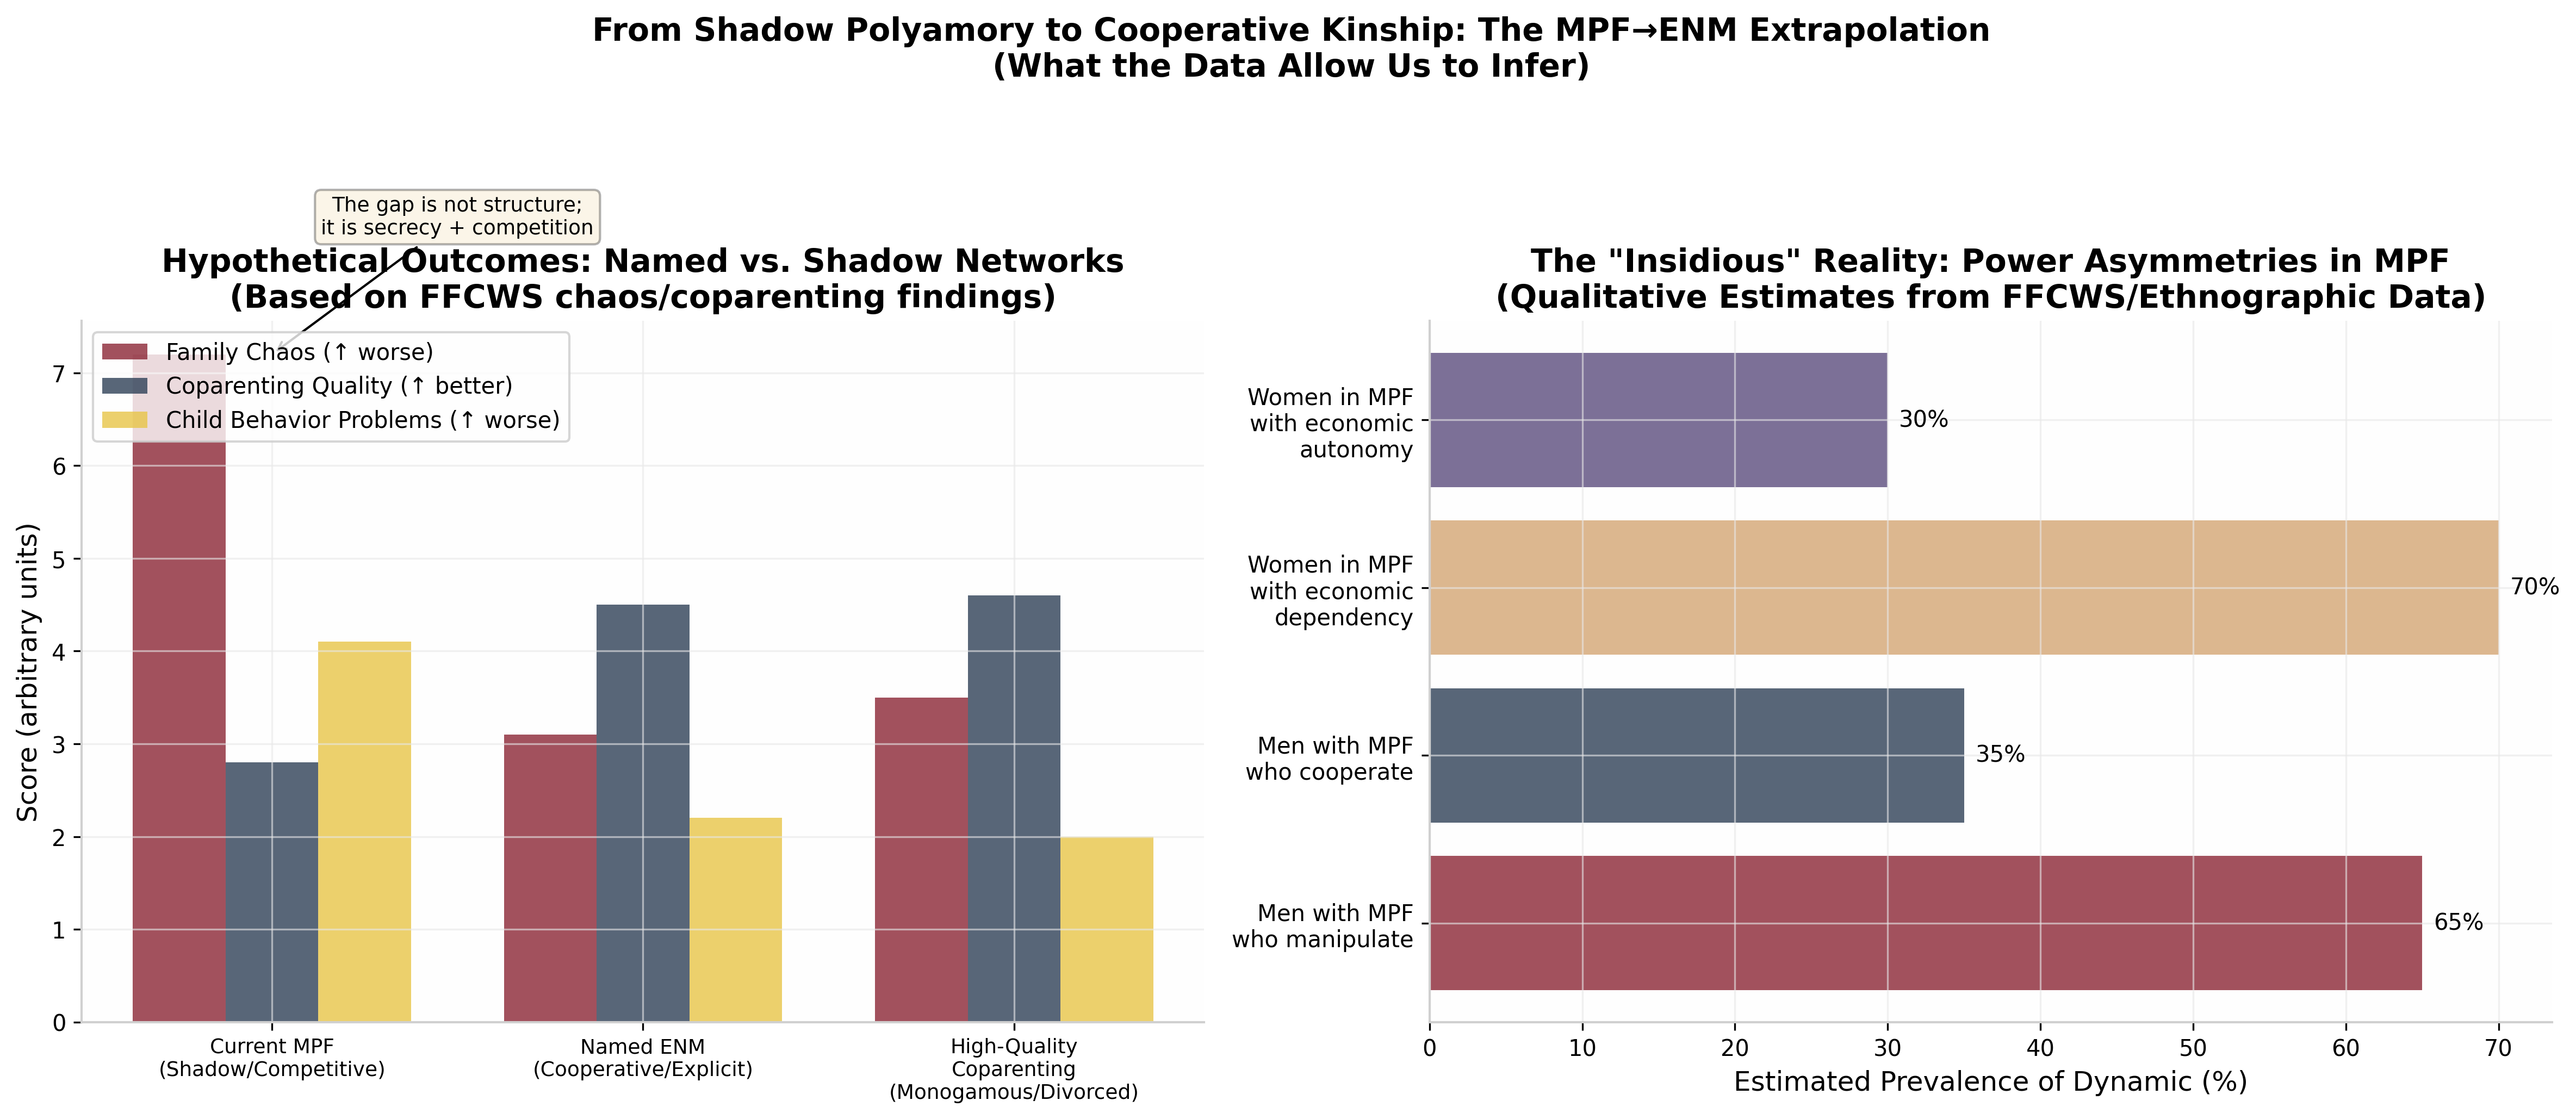
\includegraphics[width=\textwidth]{figures_mpf_enm_extrapolation.png}
  \caption{From Shadow Polyamory to Cooperative Kinship: The MPF$\rightarrow$ENM Extrapolation. Left panel: hypothetical outcomes for current MPF (shadow/competitive), named ENM (cooperative/explicit), and high-quality coparenting (monogamous/divorced) based on FFCWS chaos and coparenting findings. Right panel: estimated prevalence of power asymmetries in MPF from FFCWS and ethnographic data.}
  \label{fig:mpf_enm}
\end{figure}

\subsubsection{The ``Insidious'' Reality: Power Asymmetries}

In current MPF structures, some men actively pit women against each other to maintain control while under-providing. In the FFCWS, fathers with MPF are significantly more likely to have incarceration histories (61\% vs.~28\%), drug use, and lower earnings. ``Swapping families'' is a documented pattern: fathers reduce investment in prior children when they form new unions, often because new partners demand exclusive loyalty and resources. Loyalty conflicts are structurally incentivized: mothers with MPF report depression and stress because they must choose between protecting children from prior unions and maintaining harmony with new partners.\SourceNote{FFCWS MPF and investment pattern analyses.}

This manipulation is not a ``Black male pathology.'' It is a rational strategy under patriarchal poverty: when a man has limited resources and multiple children by multiple women, pitting the mothers against each other prevents them from collectively demanding accountability. When child support is assigned as a percentage of income that exceeds actual earnings, evasion becomes survival. When stigma prevents mothers from cooperating, they cannot pool resources to offset his underpayment.

\subsubsection{What Cooperative Kinship Would Require}

The peer-reviewed literature supports the core claim that distributed caregiving reduces individual burnout and teaches children consent and communication values. The ``sex with ex'' study found that continued sexual/romantic contact is psychologically protective when attachment persists.\SourceNote{Peer-reviewed study of 137 separated couples; CNM parenting study.} But the extrapolation is not proven, and it is not scalable without:

\begin{enumerate}
  \item \textbf{Economic autonomy for women.} No cultural shift in jealousy or stigma will work if women are economically dependent on the men they are supposed to ``cooperate'' with. The FFCWS data show that mothers who worked before the focal birth were more likely to have MPF---suggesting economic activity enables network formation.
  
  \item \textbf{State reform of child support, welfare, and custody.} Even if jealousy were unlearned, welfare marriage penalties, child support debt, and custody courts still punish multi-adult households.
  
  \item \textbf{Explicit historical trauma acknowledgment.} Cooperative non-monogamy cannot be imposed as a ``solution'' on communities that have experienced reproductive coercion. It must emerge from community-controlled frameworks where women retain full bodily autonomy and economic independence.
  
  \item \textbf{Community control rather than top-down imposition.} Because enslavers legally denied Black marriages and sold family members apart, Black communities developed fictive kin and informal care networks. Formal, named, ``legitimized'' structures may trigger suspicion of state surveillance or control.
\end{enumerate}

The MPF data allow us to hypothesize that named, cooperative, sexually-integrated multi-partner networks could produce better outcomes than shadow MPF, because the harms of MPF are driven by chaos, secrecy, and competition rather than by multiplicity itself. But this extrapolation is not proven. The framework is most powerful not as a ``solution'' to MPF, but as a theory of what MPF could become if the structural forces that currently fracture it were removed and the stigma that prevents cooperation were lifted.

\subsection{Historical Trauma and Modern Stigma}

Enslaved Black women were subjected to systematic reproductive coercion that included forced reproduction (``breeding'') between enslaved men and women to produce laborers; rape by enslavers, overseers, and slave drivers as a wealth-maximization strategy; medical experimentation without anesthesia or consent; forced wet-nursing of white infants; and punishment for infanticide or stillbirth. This was not ``bad history.'' It was a centuries-long system of reproductive terrorism that denied Black women bodily autonomy, sexual self-determination, and the right to form and protect their own families.\SourceNote{Historical scholarship on slavery, reproductive coercion, and medical experimentation.}

The stereotypes that plague Black family discourse today are direct descendants of this history. Joy DeGruy's theory of Post-Traumatic Slave Syndrome argues that centuries of chattel slavery followed by institutionalized racism produced multigenerational adaptive behaviors---some resilient, some destructive. The epigenetic transmission of stress may affect how subsequent generations experience trust, attachment, and bodily autonomy.

This history creates three specific barriers to cooperative kinship:

\begin{itemize}
  \item \textbf{Bodily autonomy suspicion.} When a structure asks Black women to share sexual/romantic access across a network, it triggers historical memory of coerced sexual availability. The ``no kids'' filter on dating apps is not just about preference; it is about protecting reproductive autonomy in a culture that has historically denied it.
  
  \item \textbf{Maternal competition as survival.} Enslaved women sometimes competed for the limited protections available to mothers (better food, lighter labor). This history may amplify the intrasexual competition seen in modern MPF, where women are structurally pitted against each other for scarce male resources.
  
  \item \textbf{Distrust of formalized kinship.} Because enslavers legally denied Black marriages and sold family members apart, Black communities developed fictive kin and informal care networks. But this also means that formal, named, ``legitimized'' structures may trigger suspicion of state surveillance or control.
\end{itemize}

There is no peer-reviewed evidence that slavery-era forced reproduction created different incest taboos in modern Black communities. Black communities generally maintain strong incest taboos and strong child-protection norms. The ``village'' model of childrearing includes surveillance and protection of children by multiple adults. However, the historical denial of Black kinship by enslavers may have contributed to the strength of fictive kin---because biological kinship was weaponized, Black communities developed chosen kin networks that were more flexible and protective than blood-based models.

\subsection{Synthesis: What the Data Actually Show}

The correct headline, based on the peer-reviewed literature, is not ``Black Men Are Deadbeats'' or ``Black Women Are Too Independent.'' It is:

\begin{quote}
Federal housing policy poisoned Black children with lead; the criminal justice system incarcerated their fathers for the resulting behavioral symptoms; the child support system trapped those fathers in debt; and welfare policy made formal marriage economically irrational. The result is family instability that is then blamed on the victims.
\end{quote}

Black family instability in America is not a gender war. It is a policy war. The same state mechanisms---mass incarceration, environmental racism, predatory child support, and punitive welfare policy---attack Black men and Black women from different angles, producing outcomes (nonresident fatherhood, single motherhood, MPF) that are then misread as individual moral failures. The ``tension'' between Black men and women is not the cause of family breakdown; it is the scar tissue left by shared structural violence.

The peer-reviewed data reject the ``small subset of irresponsible men'' narrative. Instead, they reveal cascading structural disadvantage: concentrated poverty plus lead exposure damages neurodevelopment in Black children of both sexes. For boys, this increases contact with the criminal justice system (mostly for non-violent offenses), which removes them from households and destabilizes partnerships. For girls, the same lead burden increases pregnancy complications and reduces relationship stability via partner incarceration. The result is that a large minority of disadvantaged Black men experience MPF, and a large minority of disadvantaged Black women experience single motherhood and MPF---not because of a tiny ``player'' elite, but because the same structural forces hit both sexes from different angles and produce family instability as an output.

Any honest analysis of Black families must begin with the state, not the culture. The data are unambiguous: when you control for structure (incarceration, lead exposure, unemployment, housing segregation), the racial gaps in family formation shrink or disappear. What remains is not a ``Black problem'' but an American policy problem that happens to fall heaviest on the people American policy has always targeted.
